%%This is a very basic article template.
%%There is just one section and two subsections.
%\documentclass{article}


\documentclass[a4paper,twoside]{article}

\usepackage{icgst}
\usepackage{algorithm}
\usepackage{algorithmic}

%\documentclass[preprint,12pt]{elsarticle}
%\journal{Jornal Name in the document\ldots\ldots\ldots.}
\begin{document}

% ICGST LaTeX Template
\twocolumn[
\scalebox{1.00}{
\includegraphics[width=1.00\textwidth]{pics/aimlhead}}
\title{ A Hybird Particle Swarm clustering Algorithm for Face Recognition}
\vspace{0.1in}
\author{}
\begin{center}
Maha El Meseery, Mahmoud fakhr el Deen, Heba El Nemer\\
\textit {Electronic Research Institute, Cairo, Egypt}\\
{[melmeseery, mk, heba]@sci.eri.eg},\\
\texttt{http://www.sci.eri.org}
\end{center}
\vspace{0.25in}
]
% AIML ICGST LaTeX Template


\begin{abstract}
%% Text of abstract

This paper introduce a system that recognize faces using a hybrid clustring algorithm that combines Particle Swarm Optimization and Nelder Meed modification. The PSO shows that it successfully converge during the initial global search stages to around global optimum. The recongition problem is converted into a clustering problem where each face in the database is represented with a single cluster. The paper uses two datasets to achieve results that indicates the efficency of the system. The results shows that the system gives better result compared to K-means clustering or using  linear classifier.

 %PSO algorithm was showed to
%successfully converge during the initial stages of a global search, but around
%global optimum

%where the faces in the database are grouped into clusters using the proposed
% algorithm. When a new face is introduced to the system, the system tries to
% identify the cluster that the face belong to and recognize the face based on
% the cluster
%
\end{abstract}

%\textit{\textbf{Keywords:} Autonomous robot, Stochastic control, Kalman filter,
%Fuzzy logic, Neural Network, Adaptive navigation.}ir

%\journal{Jornal Name in the document\ldots\ldots\ldots.}
\begin{frontmatter}


\title {Face recgontion using Particle Swarm clustering  }


\author[label]{Maha El Meseery}
\author[label]{Mahmoud fakhr el Deen}
\author[label]{Heba Nemer}

\address[label]{Electronic Research Institute, Cairo, Egypt}


% AIML ICGST LaTeX Template


\begin{abstract}
%% Text of abstract

This paper introduce a system that recognize faces using a hybrid clustring algorithm that combines Particle Swarm Optimization and Nelder Meed modification. The PSO shows that it successfully converge during the initial global search stages to around global optimum. The recongition problem is converted into a clustering problem where each face in the database is represented with a single cluster. The paper uses two datasets to achieve results that indicates the efficency of the system. The results shows that the system gives better result compared to K-means clustering or using  linear classifier.

 %PSO algorithm was showed to
%successfully converge during the initial stages of a global search, but around
%global optimum

%where the faces in the database are grouped into clusters using the proposed
% algorithm. When a new face is introduced to the system, the system tries to
% identify the cluster that the face belong to and recognize the face based on
% the cluster
%
\end{abstract}

%\textit{\textbf{Keywords:} Autonomous robot, Stochastic control, Kalman filter,
%Fuzzy logic, Neural Network, Adaptive navigation.}ir



\begin{keyword}
My first keyword \sep keyworbd\ldots

\end{keyword}

\end{frontmatter}

\section{Introduction}

Face recognition have become one of the most extensively studied research topics that spans different disciplines such as pattern recognition, image processing and artificial intelligence. This is due to its importance to various application like identity authentication, surveillance and intelligents vision. One of the ost used method is Eigenfaces which is used to extract relevant facial information from faces to used as features to identificy faces\cite{Turk91}.

A lot of algorithms were introduced to solve face recognition problem \cite{apperance2003,survey2003}. Several system used evolutionally algorithms like GA \cite{ga2004}.  In \cite {Ramadan2009} introduced a system that uses Particle Swarm Optimization to select features for face recognition.  Others like \cite{Wei20114390} used PSO to select best paramters of the Support vector classifier used in classification methods. In all of these application PSO was not used as the classifier or the recognizier. %ost of these system the PSO is used as anm  %was also used as feature extraction algorithm in fac The use of evolutionally algorithms in face recognition is limited

The clustring algorithm is widely used to cluster information in data and text mining and many other application. The use of clustring algorithm in classificatin was also reproted in \cite{Bagirov03unsupervisedand} where k-means algorithm is used to create clusters that are used to label input samples using some kind of distance functions. % any measure label on the input samples to one of the trained clusters.

The use of Particle swarm optimization (PSO) in data clustring was introduced by Merwe and Engelbrechet \cite{psoclustering,Cheo2004}. They presented a system that was tested on three different dataset and achieved better clustring than other clustring algorithms. Several enhancment has been added to the PSO algorithms to improve its efficiency and quality of the global solution. Several other search method like Nelder-Mead \cite{neldermead}  were also  integrated to the PSO algorithm. The use of Nelder-Meed search in the PSO proofed to enchance the quality of the global optimium solution with little computational cost \cite{nelderMeadPSO}.


In this paper we introduce a novel face recognition algorithm that uses a Particle swarm optimization (PSO) to create clusters of faces in the database. The Nelder Meed enchancment is integarted into the PSO algorithm to create clusters where Each cluster represents a single person in the database.  The first step of the system is preprocessing the database to detect and normalize the face inside the image. Secondly, feature vectors are extracted by computing the  Eigenfaces for every person in the database then extracting the wieght vector for each sample in the database. After that the training set is used to create clusters for the PSO clustering algorithm. The global solution should represents a defined center for all clusters where each cluster represent a single person. The problem of recognition of test sample is converted into measurin the distance between clusters and the input sample, the  sample will belong to the cluster with the minimum distance . % widentifying the cluster that the input sample belogs to. % step  %and the eigen vector are extracted. The  and





The remaining of the paper is organized as follows. Firstly, section \ref{sec:section2} gives the basic background infromation on  Eigenfaces, Particle swarm optimization,and Nelder Meed modification Section \ref{sec:proposed} describes in details our proposed system. Section \ref{sec:Results} presents the experiments undertaken to develop the system and also some experiments to evaluate the recognition performance of the proposed system. Finally, in section \ref{sec:Conclusion} we present conclusion and future works.

\section{Background Information}
\label{sec:section2}
In this section we will describe the basic information that is required to explain our proposed system.  We will start by explaining how to compute Eigenfaces then proceed to explain the general Particle swarm algorithm and the Nelder-Mead Modification.

\subsection{Eigenfaces}
\label{facereg}
A set of eigenfaces \cite{Turk91} can be generated by performing a mathematical process called principal component analysis (PCA) on a large set of images depicting different human faces. Informally, eigenfaces can be considered a set of "standardized face ingredients", derived from statistical analysis of many pictures of faces. Any human face can be considered to be a combination of these standard faces.

 The aim is to represent a face as a linear combination of a set of basis images called eigenfaces. That is :
\begin{equation}

\Phi _i  = \sum\limits_{j = 1}^K {\omega _i u_j }
\end{equation}

Where $\Phi_i$ represents the $i^{th}$ face with the mean subtracted from it, $\omega _i$ represent weights and  $u_j$ the eigenvectors.
This can be represented aptly in a figure as:

\begin{figure}[h]
 \begin{center}
 \centering
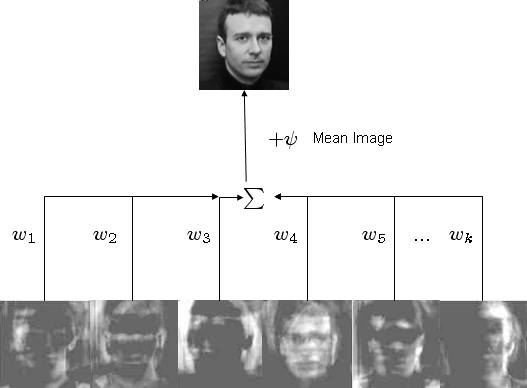
\includegraphics[scale=0.3]{eigenfacesrec.jpg} \caption{Face reconstruction from Eigenfaces. }
 \end{center}\end{figure}

There are some main assumption we have to take in account before computing the eigen computatioan and it as follows :%in computing eigen faces and it is
%\subsubsection{Assumptions:}
\begin{enumerate}

\item There are $M$ images in the training set.

\item There are $K$ most significant Eigenfaces using which we can satisfactorily approximate a face. Needless to say $K <M$.

\item All images are $NxN$ matrices, which can be represented as dimensional vectors. The same logic would apply to images that are not of equal length and breadths. To take an example: An image of size $112 x 112$ can be represented as a vector of dimension 12544 or simply as a point in a 12544 dimensional space.
\end{enumerate}
\subsubsection{Algorithm for Finding Eigenfaces}

\begin{enumerate}
\item Obtain $M$ training images , $I_1, I_2 \dots I_m$  , centered faces images.

%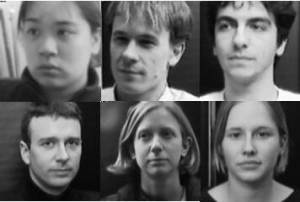
\includegraphics{training-images.jpg}
\begin{figure}[h]
 \begin{center}
 \centering
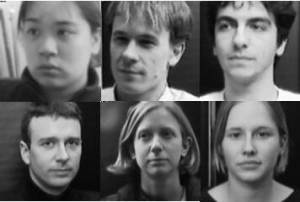
\includegraphics[scale=0.3]{training-images.jpg} \caption{Sample Faces. }
 \end{center}\end{figure}
\item Represent each image $I_i$ as a vector $\Gamma_i$.
\begin{equation}
\label{arrequation}
I_i  = \left[ {\begin{array}{*{20}c} {a_{11} } & {a_{12} } &\ldots& {a_{1N} }  \\
   {a_{21} } & {a_{22} } &  \ldots   & {a_{2N} }  \\
    \vdots  &  \vdots  &  \ddots   & {}  \\
   {a_{N1} } & {a_{N2} }  & {} & {a_{NN} }  \\
\end{array}} \right]_{NxN} \Rightarrow\left[
{\begin{array}{*{20}c}
   {a_{11} }  \\
   {\vdots}  \\
    {a_{1N} }  \\
     {a_{21}}  \\
        {\vdots}  \\
   {a_{2N} }  \\
   {\vdots}  \\
   {a_{NN} }  \\
\end{array}} \right]_{N^2 x1} = \Gamma _i
\end{equation}
\item Find the average or the mean face vector  $\Psi$

\begin{equation}
\Psi  = \frac{1}{M}\sum\limits_{i = 1}^M {\Gamma _i }
\end{equation}
\item  Subtract the mean face $\Psi$ from each face vector $\Gamma_i$ to get a set of vectors $\Phi_i$. The purpose of subtracting the mean image from each image vector is to be left with only the distinguishing features from each face and (removing)  in a way information that is common.
\begin{equation}
\Phi _i  = \Gamma_i  - \Psi
\end{equation}
\item  Find the Covariance matrix $C$:
\begin{equation}
C = AA^T
\end{equation} , where $A = \left[ {\begin{array}{*{20}c}
   {\Phi _1 } & {\Phi_2} & {\dots} & {\Phi _M }  \\
\end{array}} \right]
$
Note that the Covariance matrix has simply been made by putting one modified image vector obtained in  one column each.

Also note that $C$is a $N^2xN^2$ matrix and $A$ is a $NxM$ matrix.


\item  Instead of the Matrix $AA^T$  consider the matrix $A^TA$ .


\item Find the $M$ best  Eigenvectors of $C=A^TA$. using the relation of in Equation\ref{eigenu} Also keep in mind that $\left\| {u_i} \right\| = 1.$.

\begin{equation}
 \label{eigenu}
u_i=Av_i
\end{equation}

 where  $u_i$ is the eigen vector of $C$ and $v_i$ is the eigen value of the matrix $C$.

\item Select the best  Eigenvectors, the selection of these Eigenvectors is done heuristically.

\item Finding Weights:\\

The Eigenvectors found at the end of the previous section,  when converted to a matrix in a process that is reverse to that in STEP \ref{facereg}, have a face like appearance. Since these are Eigenvectors and have a face like appearance, they are called Eigenfaces. Sometimes, they are also called as Ghost Images because of their weird appearance.

Now each face in the training set (minus the mean),$\Phi_i$  can be represented as a linear combination of these Eigenvectors   $u_j$:
  \begin{equation}
\label{eqphi}
\Phi_i  = \sum\nolimits_{j = 1}^k {\omega_j u_j}
  \end{equation}
, where  $u_j$?s are Eigenfaces and $\omega_j$ are the weights and can be calculated as :
\begin{equation}
\label{weighteq}
\omega _j  = u_j^T \Phi _i
\end{equation}
Each normalized training image is represented in this basis as a vector $\Omega$.
\end{enumerate}

Equation \ref{eigenu} and \ref{weighteq} are used to compute the eigenfaces and weight equation for each face in the database.
\subsection{Particle Swarm Optimization}
\label{sec:ParticleSwarmAlgorithm}
 The main idea of \textit{Particle Swarm Algorithm (PSO)} is to represent each solution with a $N$ dimension particle from the solution space \cite{PSOFirst}. Each particle moves with a direction and velocity $v_{ij}$ based on equations \ref{eq:Swarm1} \& \ref{eq:Swarm}.

\begin{equation}
%\[
p_{ij}=p_{ij}+v_{ij},
%\
\label{eq:Swarm1}
\end{equation}

where $p_{ij}$ represent the $j$th dimension in the $i$th particle and $v_{ij}$ is the velocity of the $j$th dimension in the $i$th particle.

 \begin{equation}
v_{ij}  = v_{ij} \omega + c_1 r_1 (lbest_{ij}  - p_{ij} ) + c_2 r_2 (gbest_{ij}  - p_{ij} ),
\label{eq:Swarm}
\end{equation}
 where $\omega$ is the inertia weight parameter which controls the tradeoff between exploration and exploitation,  $lbest_{ij}$ is the local best particle, $gbest_{ij}$ is the global best particle, $r_1$ \& $r_2$ are random variables and $c_1$ \& $c_2$ are the swarm acceleration parameters.

 After each iteration the global best $g_{best}$ particle and the agent local best particle $l_{best}$are evaluated based on the maximum fitness functions of all particles in the solution space. The solution is found after achieving a specific number of iteration or after an error threshold is achieved.

 \subsection{Nelder-Mead Enhancment}

Nelder and Meed introduced the Nelder-Mead simplex algorithm which is a deriavative free  search algorithm that finds the local minimum of  function $f$ of several variables. For, more than two variable the simplex is triangle and search compares  the function values at the three vertex of the tirangle. The worst solution, the largest function $f$ value, is rejected and replaced with a new vertex. The search continues and a new triangle is formed then the process continues to generate a sequences of triangles, for which the function values at the vertices get smaller and smaller. These triangles are reduced in size and the coordinate of the best point (minimum) point is found.  The Nelder-Mead is a technique that is capable of moving a cluster of possible solutions in a gradient direction which can be very effectively combined with GA and PSO approaches. Simillar hybrid evolutionary algorithms proved to be very successful in continous optimization problems.


The Nelder-Mead smplex method makes use of a construct called a simplex When the search space is $n$-dimensional, the simplex consists of $n+1$ solutions, $s i = {1,2,\dots  , n+1}$, that are usually closely spaced. In a two-dimensional search plane, a simplex is a triangle. The fitness of each solution is considered in each step of the Nelder-Mead method, and the worst solution $w$ is identified. The centroid, $c$, of the remaining n points is computed and the reflection of $w$ along it determined. This reflection yields a new solution $r$ that replaces $w$, in the next step. If the solution $r$ produced by this reflection has a higher fitness than any other solution in the simplex, the simplex is further expanded along the direction of $r$. On the other hand, if $r$ has a low fitness compared to the others, the simplex is contracted. Contraction can be either outward or inward depending upon whether $r$ is better or worse than $w$. The contraction operations are shown in the middle right and bottom left of the figure. If neither contraction improves the worst solution in the simplex, the best point in the simplex is computed, and a collapse is then carried out, and all the points of the simplex are moved a little closer towards the best one.

\section{Proposed System}
\label{sec:proposed}

This paper presents the a face recognition system based on hybird PSO clustering algorithm. Figure \ref{Blockchart} shows the flow chart for the training and testing modules. The training is divided into three steps 1) preprocessing, 2) feature extraction and then 3) clustring using a hybird Particle Swarm Optimization. The follwoing few section will discribe in details each step.


\begin{figure}
 \begin{center}
 \centering

 \subfigure['Training']{\label{fig:block1}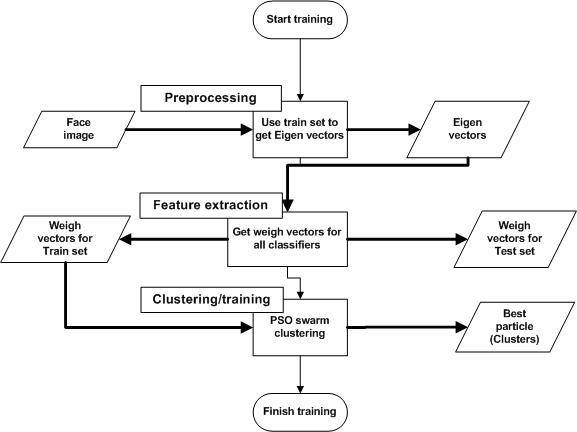
\includegraphics[width=0.45\textwidth]{block1.jpg}}
  \subfigure['Testing']{\label{fig:block2}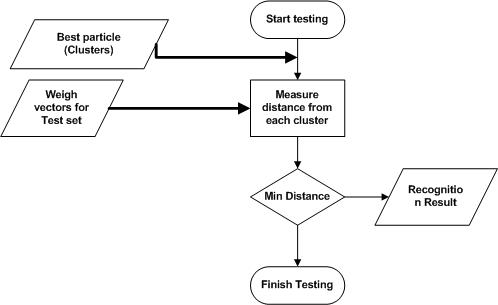
\includegraphics[width=0.45\textwidth]{block2.jpg}}

\caption{ The flow Chart}
\label{Blockchart}
 \end{center}\end{figure}
\subsection{Preprocessing}
The preprocessing step function is to detect the face from the input images then normalize and the face to the center of each  image.  Every face image in the database is  then scalled to the constant size of $h \times w$ \footnote{ note that  $h$ height and $w$ wdith are emprically choose to be 60 adn 80 respecitivily.}. The next step is computing the eigenfaces for each person in the dataset as explianed in section \ref{facereg}.


\subsection{Feature Extraction}

After the computing the eigenfaces of every person on the database the system extracts eigen weight vector for each image. Equation \ref{} shows how the weight vector is computed from the eigen faces. These weights are used as features for the clustering algorithm. The output of this stage is a dataset that contains a eigen weight vector for each face in the database which is considered the feature vector of this face.


\subsection{PSO clustering}
\label{sec:psoClustering}

The clustering algorithm is used to group the input faces into clusters which represents the persons in the dataset. The process of clustring the input faces is simillar to a classifier training in classification systems.    The clustering algorithm used is based on Particle Swarm algorithm  based on the Merwe and Engelbrechet \cite{psoclustering} Method where particle represents a possible clustering of the whole dataset.  Each particle $X_i$ is constructed such that that
\begin{equation}
X_i=\left( m_{i1}, m_{i2}, m_{i3},\dots, m_{iN_c}\right)
\end{equation}
where $N_c$ is the number of clusters to be formed and $m_{ij}$ corresponds to the $j^{th}$ centroid of the  $i^{th}$ particle, the centroid of the cluster $C_{ij}$. Thus single particle represents a candidate solution to a given clustering algorithm. Each particle is evaluated using the following equation:

\begin{equation}
F_c  = \frac{{\sum\nolimits_{j = 1}^{N_c } {\left[ {\sum\limits_{\forall z_j  \in C_{ij} } {\frac{{d(z_p ,m_{ij} )}}{{\left| {C_{ij} } \right|}}} } \right]} }}{{N_c }}
\end{equation}
where $F_c$ is the fitness function, $N_c$ is the number of clusters in the particle, $Z_p$ denotes the $p^{th}$ data vector $\left| {C_{ij} } \right|$ is the number of data vectors belonging to the cluster $C_{ij}$ and $d$ is the Euclidian distance between $Z_p$ and $m_{ij}$.

Other fitness function are also used to take into account the size of cluster and the number of elements in each cluster which improve the clustring algorithm. The two different fittness used are as follows:

\begin{equation}
F2 =  \left\{ \sum\nolimits_{j=1}^{N_c} \left[ \left( \sum\limits_{\forall z_j \in C_{ij}} d(z_p ,m_{ij} )/\left|{C_{ij} }\right| \right) \times  \left(  \left|{C_{ij} }\right| /N_o\right)\right]\right\}
\end{equation}
where $F2$ is the second fitness function, $N_o$ is the number of data vectors to cluster.

by adding considration of the cluster distribution the equation could be changed into :

\begin{equation}
F3 =  F2\times \left(\left|{C_{ik} }\right|-\left|{C_{il} }\right|+1 \right)
\end{equation}
where $\left|{C_{ik} }\right|$ is computed as $\max\forall_{j=1,2 \dots N_c}$ and $\left|{C_{il} }\right|=\min\forall_{j=1,2 \dots N_c}$


The clustering algorithm prposed can be as follows:

\begin{algorithmic}
\STATE  Generate $N$ particles with $N_c$ clusters  ($P_i,$ $\dots,$ $P_{N_c}$)
\STATE Initialize the clusters centroids for each particle randomly
\FOR{i=0 \TO $t_{max}$}
  \FOR{ each particle  $p_i$}
    \FOR{ each data vector  $zp$}
        \STATE   Calculate distance $d(zp,m_{ij})$ from cluster centroid.
        \STATE   Assign $zp$ to cluster $C_{ij}$ such that
        \STATE   $d(zp,m_{ij})=min \forall k=1,\dots,N_c {d(zp,m_{ik})}$
    \ENDFOR
    \STATE  Compute the Fitness function for the particle.
     \STATE  Update the global best and local best
     \STATE  Move all particle using PSO equations.
     \ENDFOR
  \ENDFOR
 \RETURN global best
%\end{verbatim}

 \end{algorithmic}

 Figure shows the \ref{fig:pso1} the block diagram for the PSO clustering algorithm.

\begin{figure}
 \begin{center}
 \centering
 \subfigure['PSO
 clustering ']{\label{fig:pso1}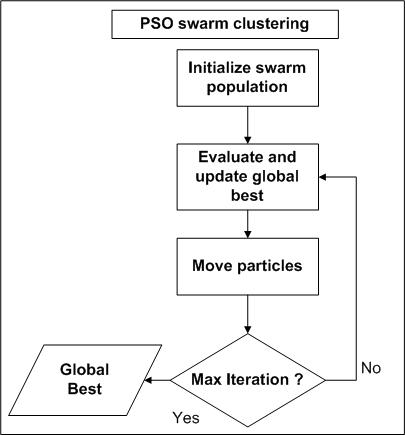
\includegraphics[width=0.25\textwidth]{pso1.jpg}}
 \subfigure['Nelder
 meed a']{\label{fig:pso2}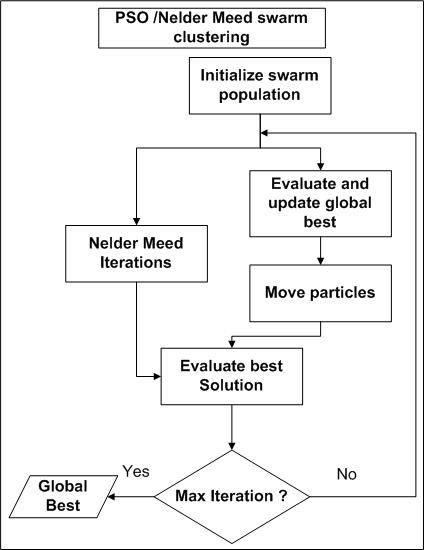
\includegraphics[width=0.25\textwidth]{pso2.jpg}}
  \subfigure['Nelder
  meed b']{\label{fig:pso3}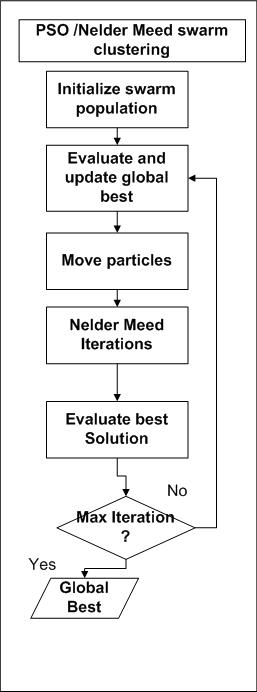
\includegraphics[width=0.25\textwidth]{pso3.jpg}}
\caption{ Particle Clustering Alogirhtm}
\label{fig:PSOswarm}
 \end{center}\end{figure}


The PSO algorithm is used to clusters each face weights computed using equation \ref{weighteq}. The algorithms first compute the eigen vectors for all faces in the database as explained in section \ref{facereg}. The computed $u_j$ Eigen vectors is used to compute the weights for each input image in the database. The clustering algorithm is used to get center weigh vector for each person. %I choose the number of clusters same as number of person for easier recognition step.


Integrating the PSO clustering algorithms with the Nelder Mead algorithm is done using either using Nelder-Mead in a parallel iterative process with the PSO as in figure \ref{fig:pso2}. Figure \ref{fig:pso3} shows a sequencial integration of Nelder-Mead search method inside the PSO algorithm where after each iteration of the PSO a single interation of Nelder-Mead is performed to improve the solution. Both mehtods are embeded in the system and comparison  between both of them is presented in \ref{sec:Results}, % After the PSO clustering algorithm is constructed two d


The recognition step will be easier as to compute the weigh vector of the input image and then compute the distance from each cluster centroid. The cluster with the min distance is the cluster of the face.

\section{Results}
\label{sec:Results}
Two different databases  was processed, the first contains 60 indian faces frome the indian face database \cite{JainMukherjeeIndianFaceDB} with 11 different samples per person  with different poses, lighting conditions and experisions. The second database is 120 eroupian faces from database \cite{} with 20 different samples per person. Both databases are processed to normalize the input to the algorithm. The dataset is then divided into training and testing set by dividing the samples of each person to either training or testing.  Four different  random training - testing splits generate the result of the following experiments . The recognition result presented is the average of the four runs of the four different splits. In the next section recognition rate is number of corrrectly identified input images over the total number of face in the testset.


\subsection{Experiments Finding PSO paramters}
\label{sec:pso}

Particle swarm consist of many paramters that controls how the search is operated and have direct impact on the output of the system. Table \ref{tab:PSO1} shows the result of different PSO paramters $c_1,c_2,W$. The result gives the indication that the swarm moves quickly to the global best by the effect of $c2$ is more improtant than $c1$.

\begin{table}
	\centering
		\caption{PSO Result }
	\label{tab:PSO1}
	%\scalebox{0.99}{
		\begin{tabular}{|l|c|c|c|c|c|}
		 \hline
C1 &	1	&1.2&	1.6&	1.8 &	2	\\ \hline
	&70.893	&70.893	&70.605	&70.029	&69.741 \\  \hline
C2	&	1	&1.2&	1.6&	1.8 &	2	\\ \hline
	&70.89	&70.61	&70.89	&69.45	&69.45 \\ \hline
W	&0.5&	1	&1.5	&2&	4	\\ \hline
	&69.74	&70.89&	70.89	&70.32&	70.89	\\ \hline
\end{tabular}
		%}
\end{table}

Another experiment to determine the system paramter is the number of training smaples required to get good results. Table \ref{tab:PSOtrainTest} shows the result when the system used different number of trainig samples per person. It is clear from the results that the system show good recognition result with only few trianig samples.

\begin{table}
	\centering
		\caption{PSO Result }
	\label{tab:PSOtrainTest}
	%\scalebox{0.99}{
		\begin{tabular}{|l|c|c|c|c|c|}
		 \hline
C1 &	1	&1.2&	1.6&	1.8 &	2	\\ \hline
	&70.893	&70.893	&70.605	&70.029	&69.741 \\  \hline
C2	&	1	&1.2&	1.6&	1.8 &	2	\\ \hline

\end{tabular}
		%}
\end{table}

\subsection {Comparing With other systems}
\label{sec:comparingSystems}

The system is compared with kmeans clustering algoirthm and general eigne faces system. The kmeans algoirthm is similar clustering algorithm and provides similar classification via clustering algorithms. Eigenfacs is genearly classifieed using eculidean distance. Table \ref{tab:system} shows the result of comparing the results of the proposed systems and kmeans. The results shows that our proposed alogrithm is more superior than kmeans clustering algoirhtms.


\begin{table}
	\centering
		\caption{PSO Result }
	\label{tab:system}
	%\scalebox{0.99}{
		\begin{tabular}{|l|c|c|c|c|c|}
		 \hline
C1 &	1	&1.2&	1.6&	1.8 &	2	\\ \hline
	&70.893	&70.893	&70.605	&70.029	&69.741 \\  \hline
C2	&	1	&1.2&	1.6&	1.8 &	2	\\ \hline
	&70.89	&70.61	&70.89	&69.45	&69.45 \\ \hline
W	&0.5&	1	&1.5	&2&	4	\\ \hline
	&69.74	&70.89&	70.89	&70.32&	70.89	\\ \hline
\end{tabular}
		%}
\end{table}


The efficency of the clustring algorithm is also  tested using differen fitness functions (see section \ref{sec:psoClustering}). Table \ref{tab:fitness}  shows the result of three different fitness functions and the effect of each fitness on the final recognition rate.


\begin{table}
	\centering
		\caption{PSO Result }
	\label{tab:fitness}
	%\scalebox{0.99}{
		\begin{tabular}{|l|c|c|c|c|c|}
		 \hline
C1 &	1	&1.2&	1.6&	1.8 &	2	\\ \hline
	&70.893	&70.893	&70.605	&70.029	&69.741 \\  \hline
C2	&	1	&1.2&	1.6&	1.8 &	2	\\ \hline
	&70.89	&70.61	&70.89	&69.45	&69.45 \\ \hline

\end{tabular}
		%}
\end{table}

\subsection{ Comparing Nelder enhancement}
\label{sec:comparingSystems}
Figrue \ref{} shows two different method to add Nelder enhancment to the PSO clustering algorithm. As mentioned in section \ref{} both methods are evaluated to select best integration methods.  Table \ref{tab:nelder} shows the result of comparison between the clustering algorithm without Nelder-Mead and using two integration methods. The results show that Nelder-Mead enhancment improved the recognition accuracy. %achieve

\begin{table}
	\centering
		\caption{ Nelder enhancement  }
	\label{tab:nelder}
	%\scalebox{0.99}{
		\begin{tabular}{|l|c|c|c|c|c|}
		 \hline
C1 &	1	&1.2&	1.6&	1.8 &	2	\\ \hline
	&70.893	&70.893	&70.605	&70.029	&69.741 \\  \hline
C2	&	1	&1.2&	1.6&	1.8 &	2	\\ \hline

\end{tabular}

\end{table}

\section{Conclusion and future work}
\label{sec:Conclusion}
In this paper we introduced a system that recognize faces using a hybrid PSO clustering algorithm. The clustering algorithm is simple and achieved better result than other methods.


Our future work will focus on improving the feature extraction method by using various features like DCT and wavelet features. Another improvement is trying to use clustering algorith to problems rather than face recognition.



\bibliographystyle{plain}
%\bibliographystyle{model1a-num-names}
\bibliography{mybibfile,library}

\end{document}
